\subsection{Der Anfang, doch wie kommt man dahin ?}

Der Anfang, doch wie kommt man dahin ?


\begin{figure}[H]
	\centering
	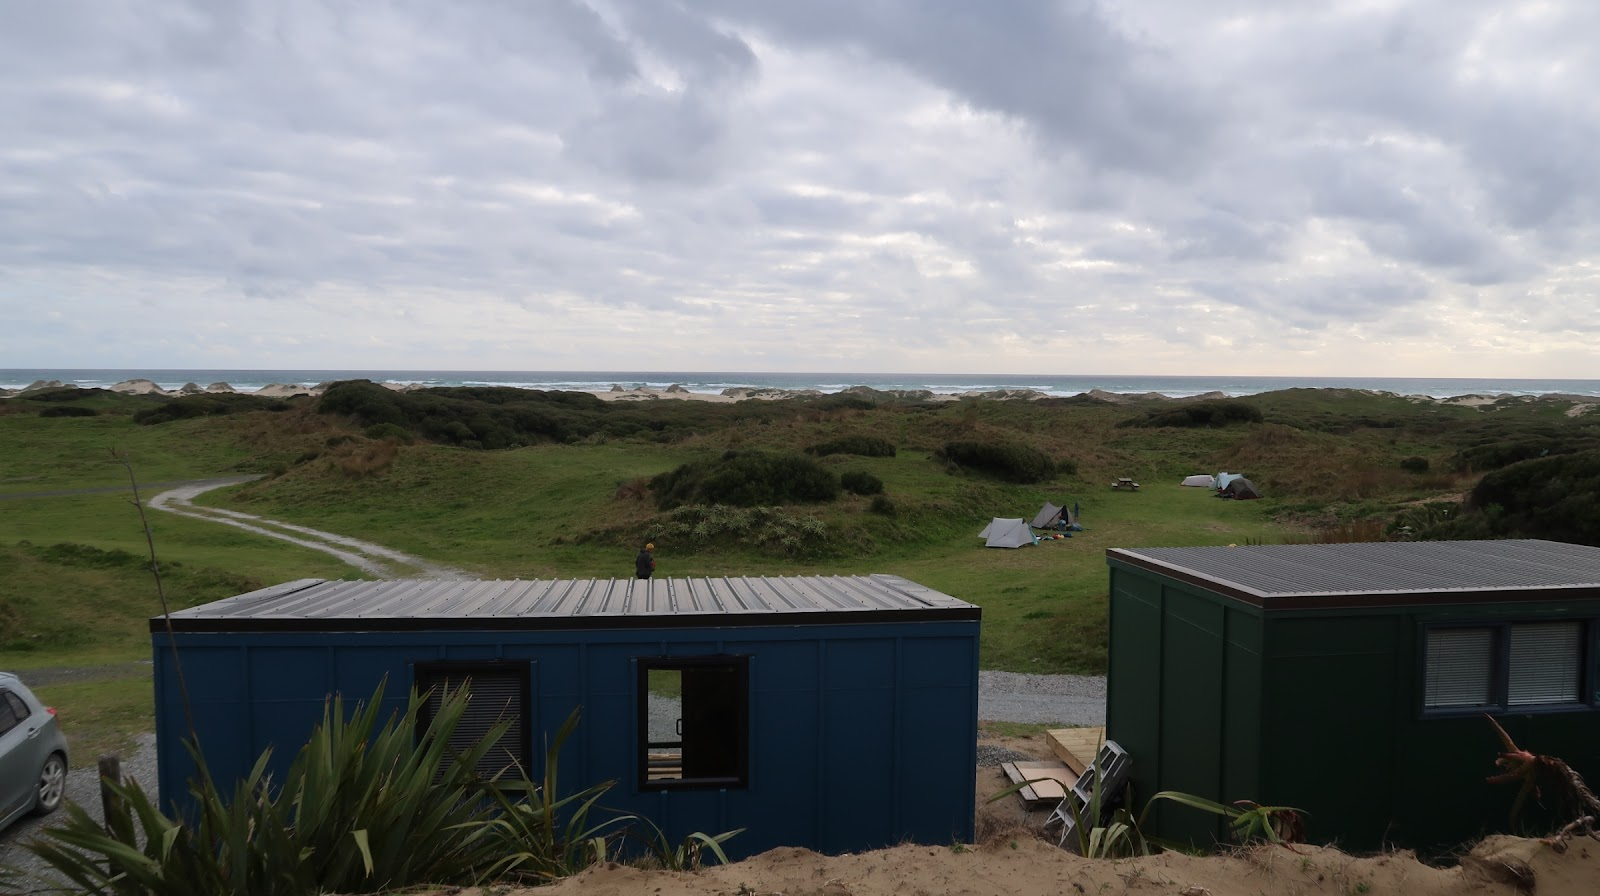
\includegraphics[width=0.5\textwidth]{der_anfang_doch_wie_kommt_man_dahin/16_1666211283532182-0.png}
	\caption{}
	\label{fig:16_1666211283532182-0}
\end{figure}

\begin{figure}[H]
	\centering
	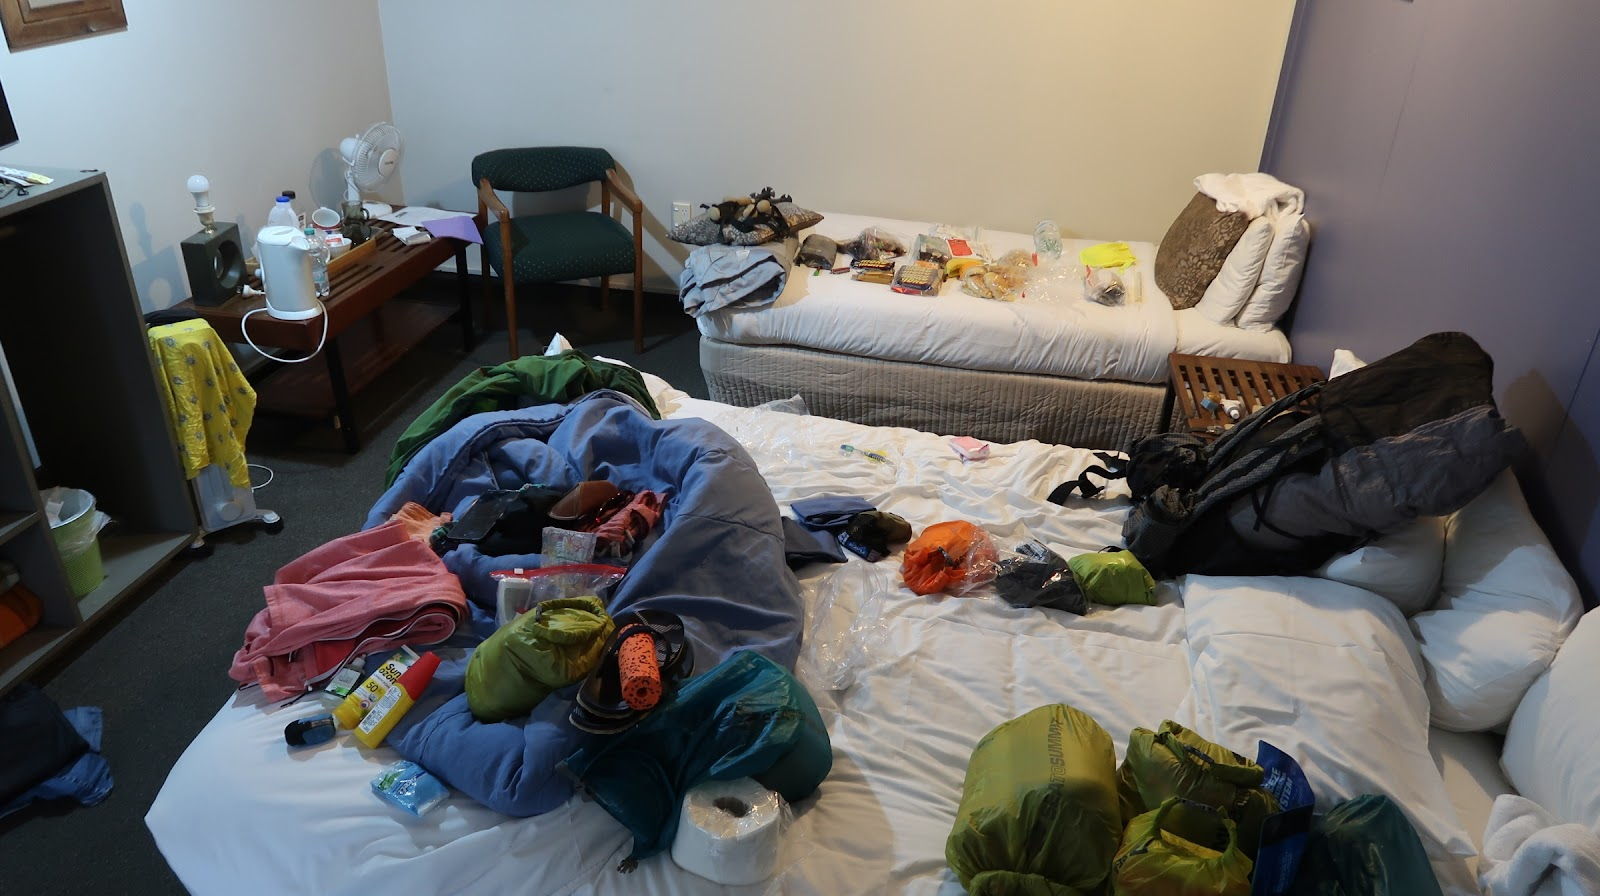
\includegraphics[width=0.5\textwidth]{der_anfang_doch_wie_kommt_man_dahin/17_1666211277698255-1.png}
	\caption{}
	\label{fig:17_1666211277698255-1}
\end{figure}

  Nach einer kleinen Verzögerung aufgrund einer nicht richtig funktionieren Neuseeländischen Handy Karte und dem Besuch zweier Handyläden, stehen wir dank einer sehr kompetenten Vodafone- NZ Mitarbeiterin schließlich mit erhobenen Daumen am Ortsrand von Kerikeri. Bereits einer der ersten PKW stopt, der Fahrer stammt hier aus Kerikeri und hat zwei Frauen abgeholt, die auch Teile des TA laufen. Er bringt uns etwa 3-4 km weiter zur Haupstrasse Richtung Awanui, hier stehen wir etwa 15 Minuten, es beginnt zu regnen, zum Glück gibt es auf der anderen Straßenseite ein Café. Nach einem etwas scheußlich Kaffee und nach Ende des Regens dauert es nur kurz und ein Rentner nimmt uns 22 km mit bis nach Kaeo. Wir werden über die Gefahr des Trampens
 


  aufgeklärt und erfahren etliches Neues über die Gegend.
 


\begin{figure}[H]
	\centering
	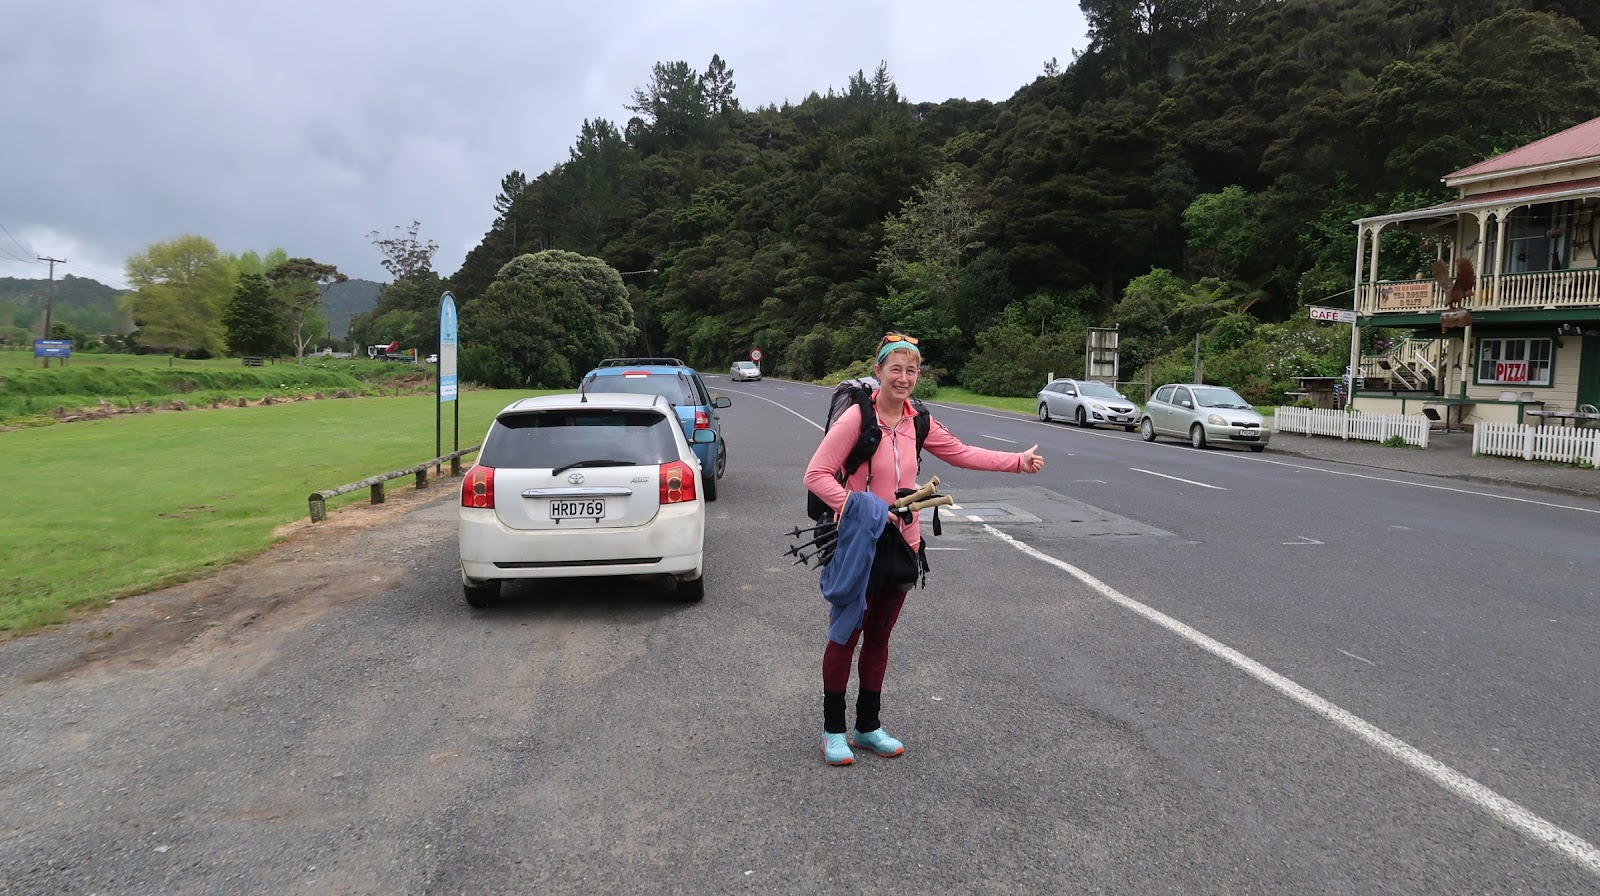
\includegraphics[width=0.5\textwidth]{der_anfang_doch_wie_kommt_man_dahin/18_1666211270506662-2.png}
	\caption{}
	\label{fig:18_1666211270506662-2}
\end{figure}

  In Kaeo dauert der Zwischenstop nur ein paar Minuten und ein Barber, der für seine beiden Söhne zwei Kayaks abholen will, nimmt uns mit nach Coopers Beach, wieder 34 km dem Ziel näher. Hier laufen wir erst einmal etwa einen Kilometer zur öffentlichen Toilette am Strand, um gerade rechtzeitig zurück zu kommen. Denn
 


  sonst hätte uns der ehemalige, ewa 80 jährige Arzt, welcher hier gerade einen Termin bei seiner Ärztin hatte,  nicht mitnehmen können. Ein wahren Glücksgriff, den die Fahrt geht bis nach Pukenui, wieder 59 km geschafft. Wir erfahren diesmal vieles über das Leben des ehemaligen Arztes seine Sammelleidenschaft (  nautische Messgeräte) und seiner Familie. Er erwähnte, dass er nebenbei eine zeitlang den öffentlichen Rettungswagen fuhr. Jetzt wird uns klar woher sein Fahrstiel kommt. Mittlerweile regnet es stärker, nach ein paar Minuten gabelt uns ein Einheimischer auf, der uns aus dem Regen retten will. Als wir ihm von unserem Vorhaben erzählen, rät er uns davor dringend ab, er schlägt uns einen Campingplatz vor, dort würde er uns hin bringen. Es schüttet mittlerweile und so kann er es auch nur schwer verstehen, dass wir sein Angebot ausschlagen. Er bringt uns trotzdem bis zu einem Laden in Te Kao, wieder 28 km geschafft. Jetzt trennen uns nur noch 44 km vom Cape. Nur wer fährt schon bei so einem schlechten Wetter dorthin... Niemand. Nach fast einer Stunde hält doch noch ein PickUp. Der Fahrer muss erst den Beifahrersitz von etlichen Müll befreien, der landet im Fussraum bei unzähligen Getränkedosen und etlichen anderen ehemaligen Lebensmitteln, ich glaube die Reste einer Pizza erkennen zu können. Macht uns natürlich nichts, Petra zwängt sich hinten zwischen verschiedenste Kanister. Unser Fahrer arbeitet als Bestäuber und bestäubt mit seinen Bienen die Avocados der umliegenden Farmen, er ist gerade auf dem Heimweg und kann uns 24 km mitnehmen. Ich frage ihn, ob er uns gegen eine kleine Spende bis zum Cape bringen könnte, er willigt gleich ein und bringt uns direkt bis zum Parkplatz vor dem Cape.
 


\begin{figure}[H]
	\centering
	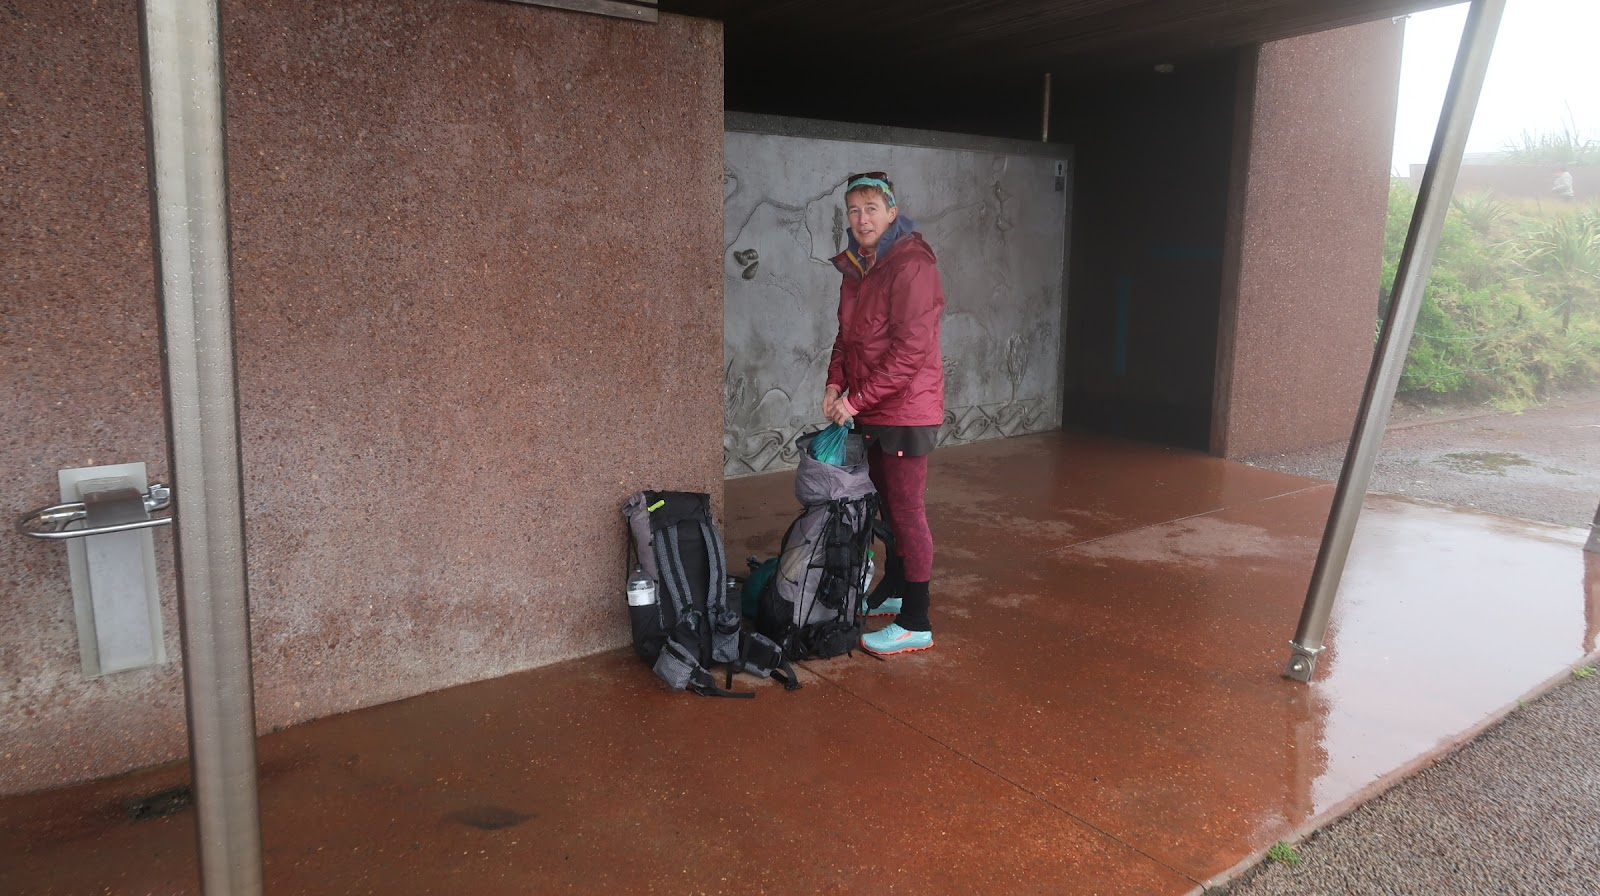
\includegraphics[width=0.5\textwidth]{der_anfang_doch_wie_kommt_man_dahin/19_1666211262307180-3.png}
	\caption{}
	\label{fig:19_1666211262307180-3}
\end{figure}

  Mittlerweile ist es fast 16:00 Uhr, etwa zur gleichen Zeit hatten wir uns  vor 4 Jahren hier auf den Weg zum Leuchtturm gemacht. Damals hätten wir nie daran gedacht noch einmal hierher zu kommen, um uns nochmals auf den langen Weg Richtung Süden zu machen.
 


  Mo 17 .10.22    Tag 1
 


  Km 0 - 12,5
 


  Cape Reinga - Twiligt Beach Camp
 


\begin{figure}[H]
	\centering
	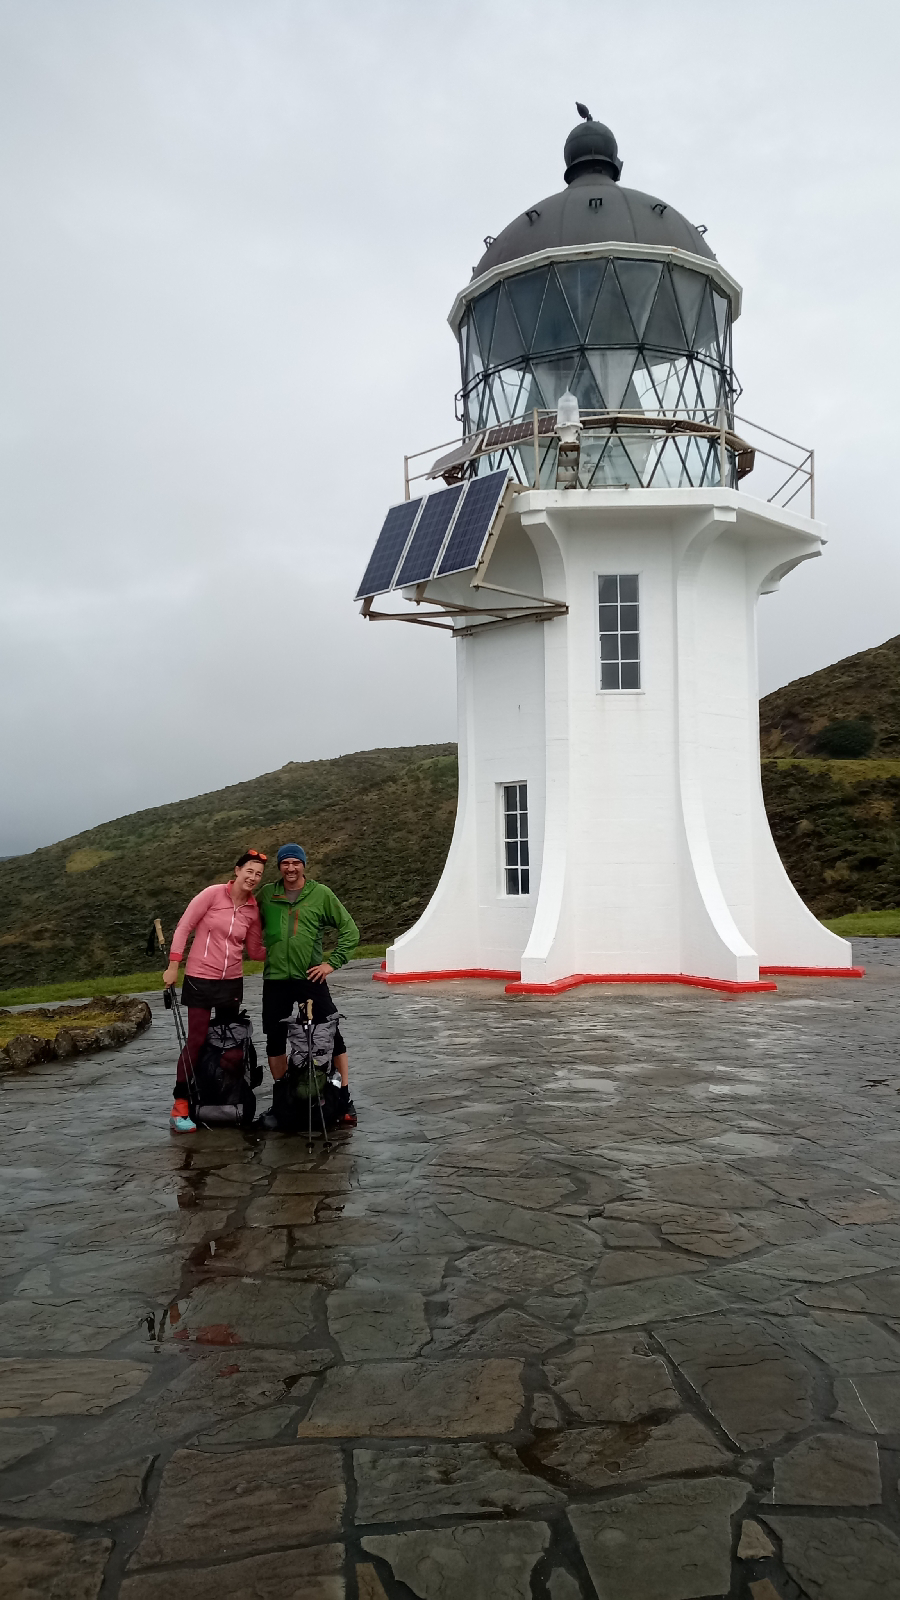
\includegraphics[width=0.5\textwidth]{der_anfang_doch_wie_kommt_man_dahin/20_1666211256578828-4.png}
	\caption{}
	\label{fig:20_1666211256578828-4}
\end{figure}

  Nach ein paar Fotos machen wir uns auf den Weg, dieses Mal wollen wir noch bis zum 12,5 km entfernen, Twilight Beach Camp laufen, beim ersten Mal kamen wir nur 6 km weit, denn dann war es schon zu dunkel.
 


\begin{figure}[H]
	\centering
	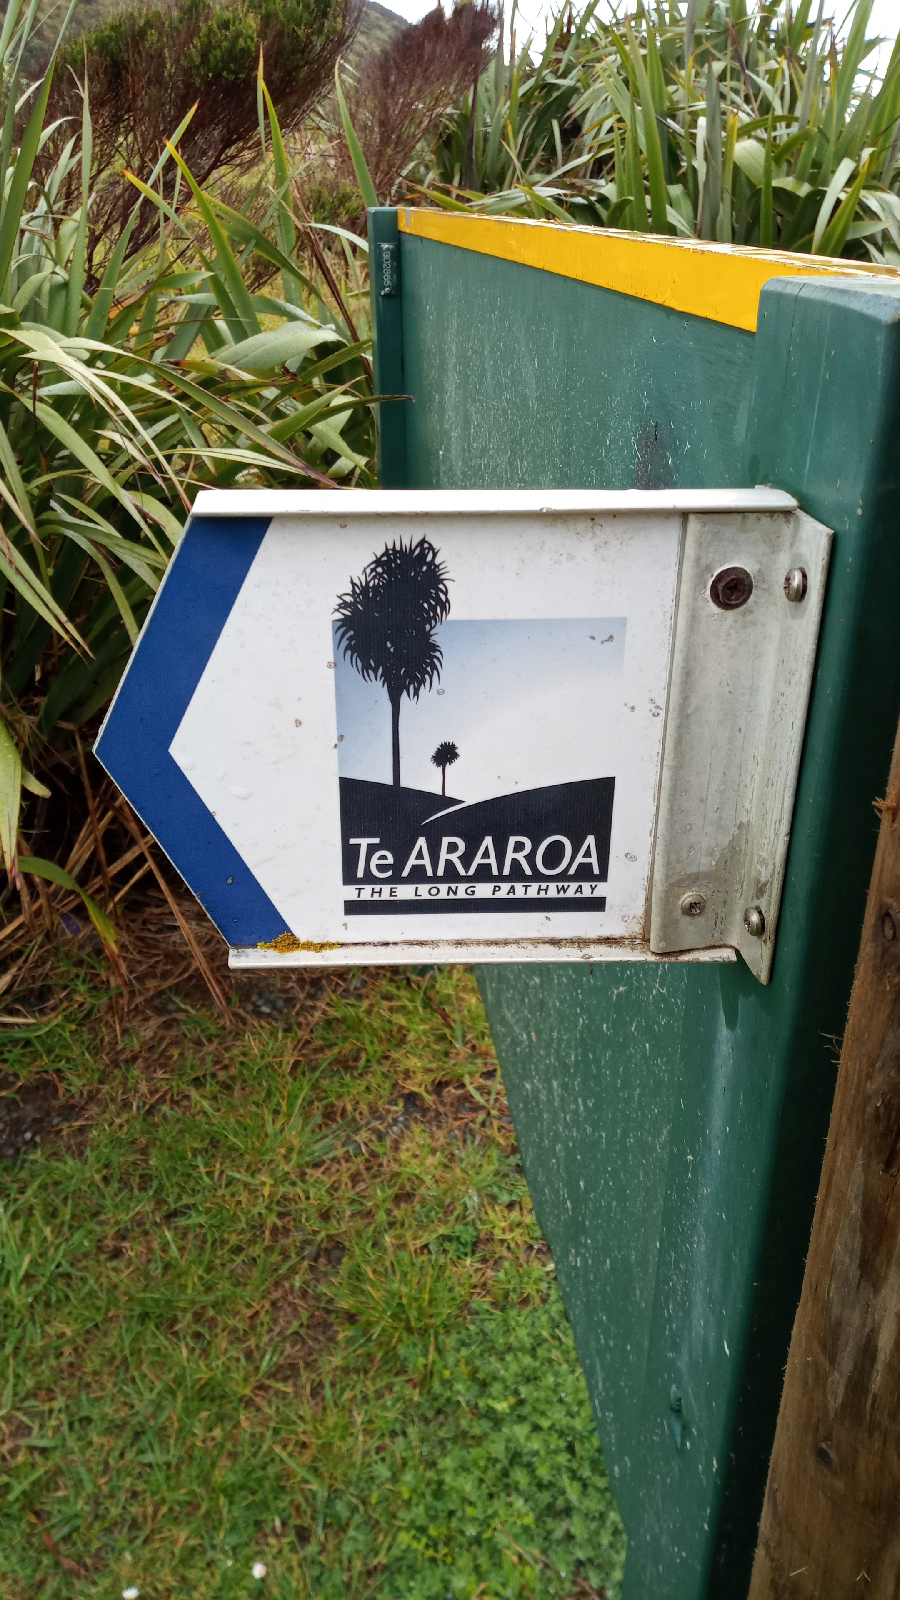
\includegraphics[width=0.5\textwidth]{der_anfang_doch_wie_kommt_man_dahin/21_1666211249426774-5.png}
	\caption{}
	\label{fig:21_1666211249426774-5}
\end{figure}

  Diese Schild werden wir hoffentlich noch oft sehen.
 


  Wir bleiben auch jetzt ständig stehen um Fotos zu machen.
 


\begin{figure}[H]
	\centering
	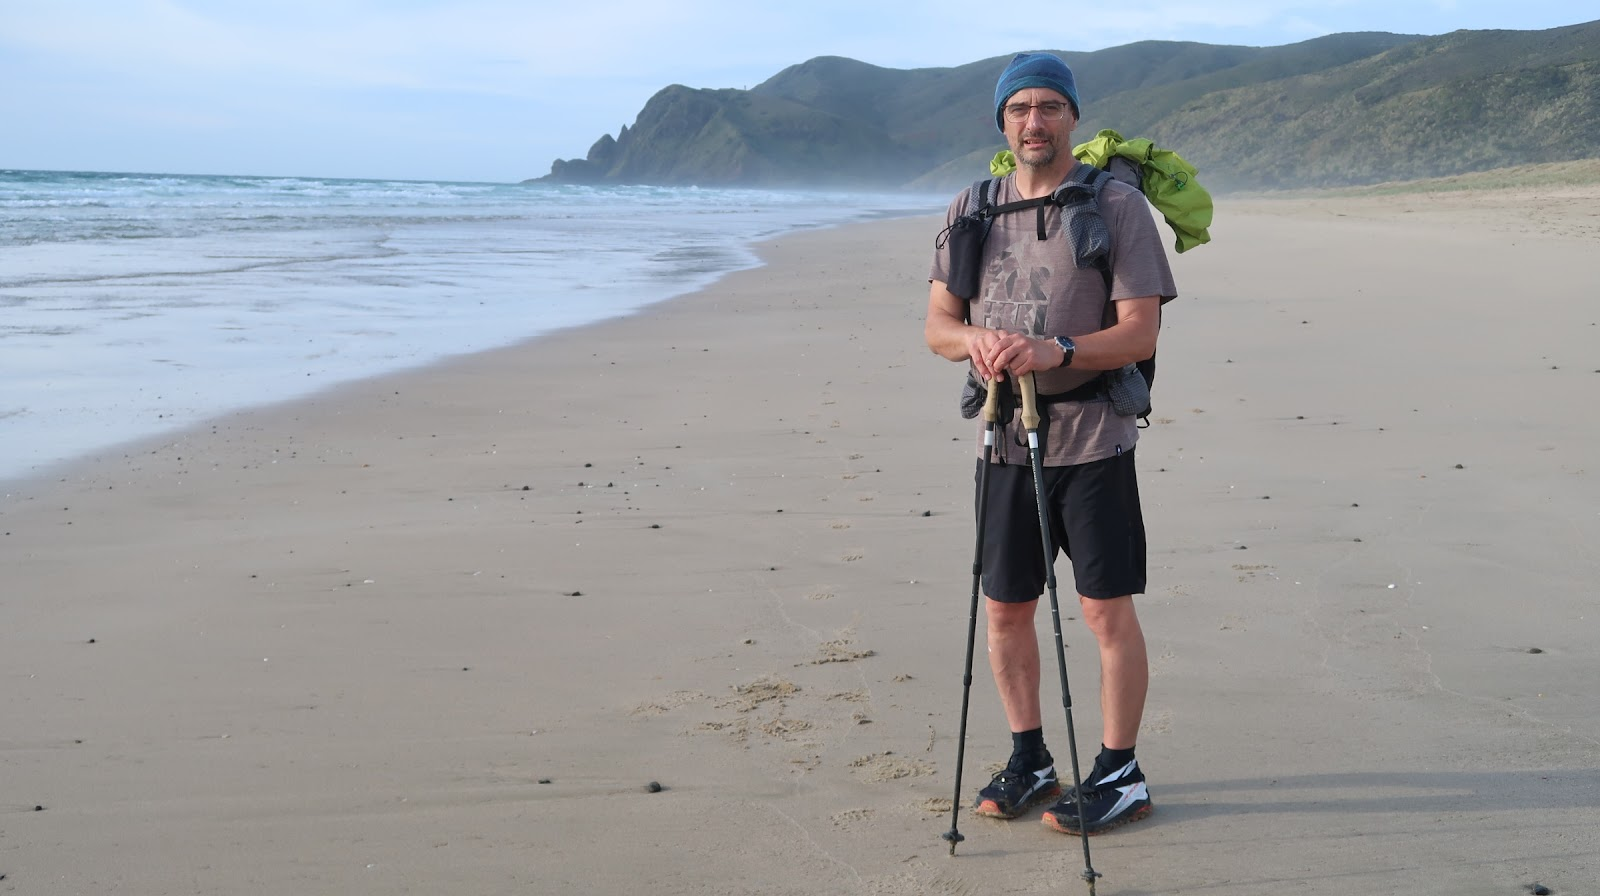
\includegraphics[width=0.5\textwidth]{der_anfang_doch_wie_kommt_man_dahin/22_1666211243190084-6.png}
	\caption{}
	\label{fig:22_1666211243190084-6}
\end{figure}

\begin{figure}[H]
	\centering
	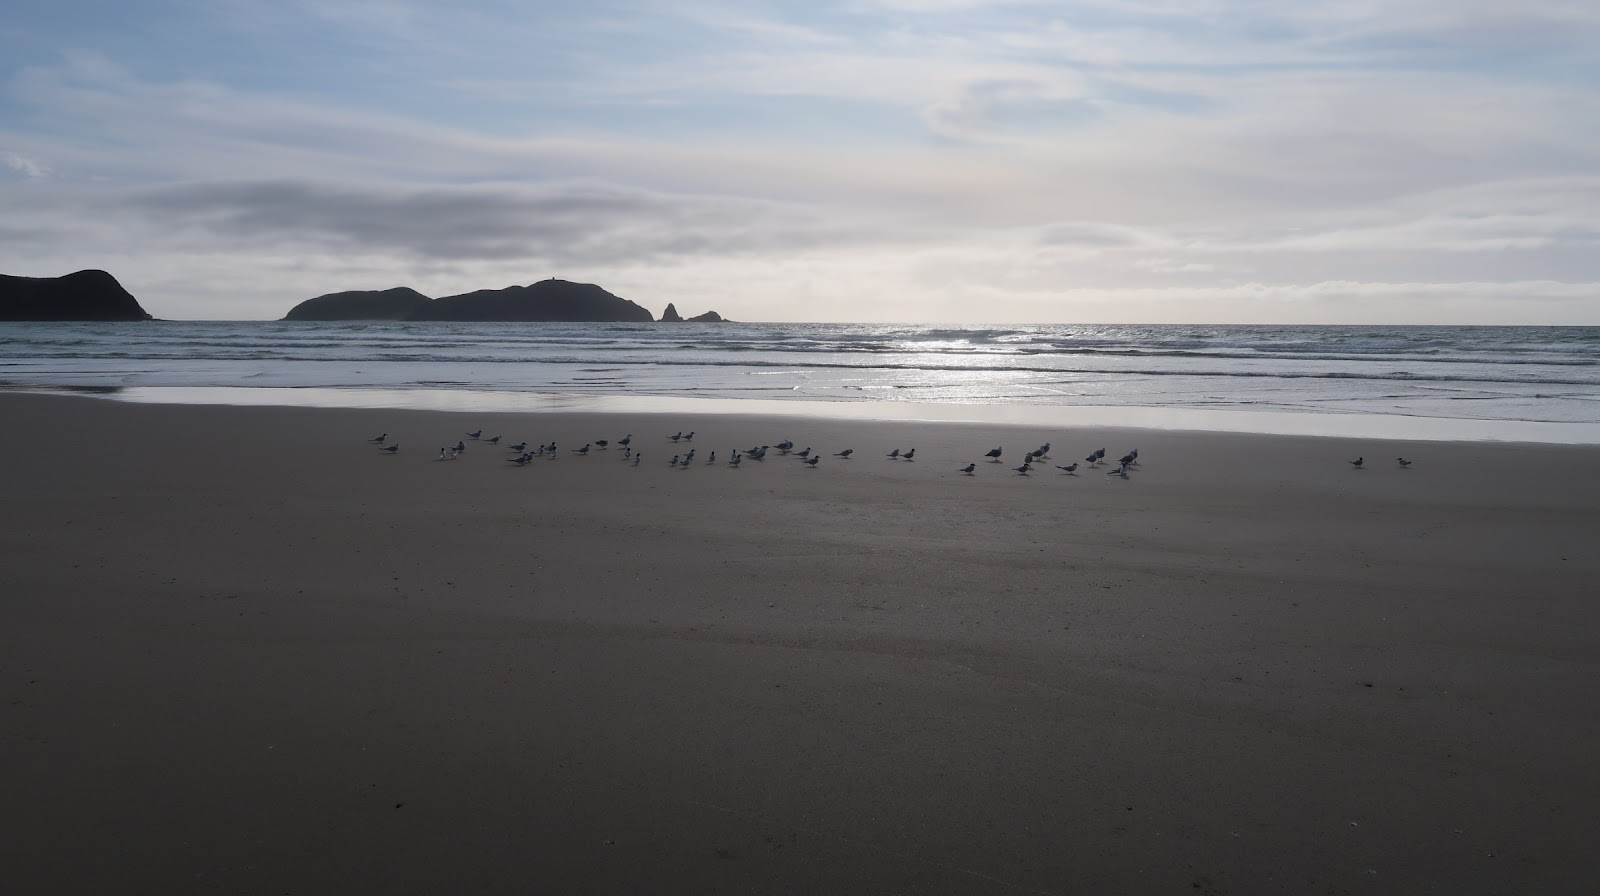
\includegraphics[width=0.5\textwidth]{der_anfang_doch_wie_kommt_man_dahin/23_1666211236677174-7.png}
	\caption{}
	\label{fig:23_1666211236677174-7}
\end{figure}

\begin{figure}[H]
	\centering
	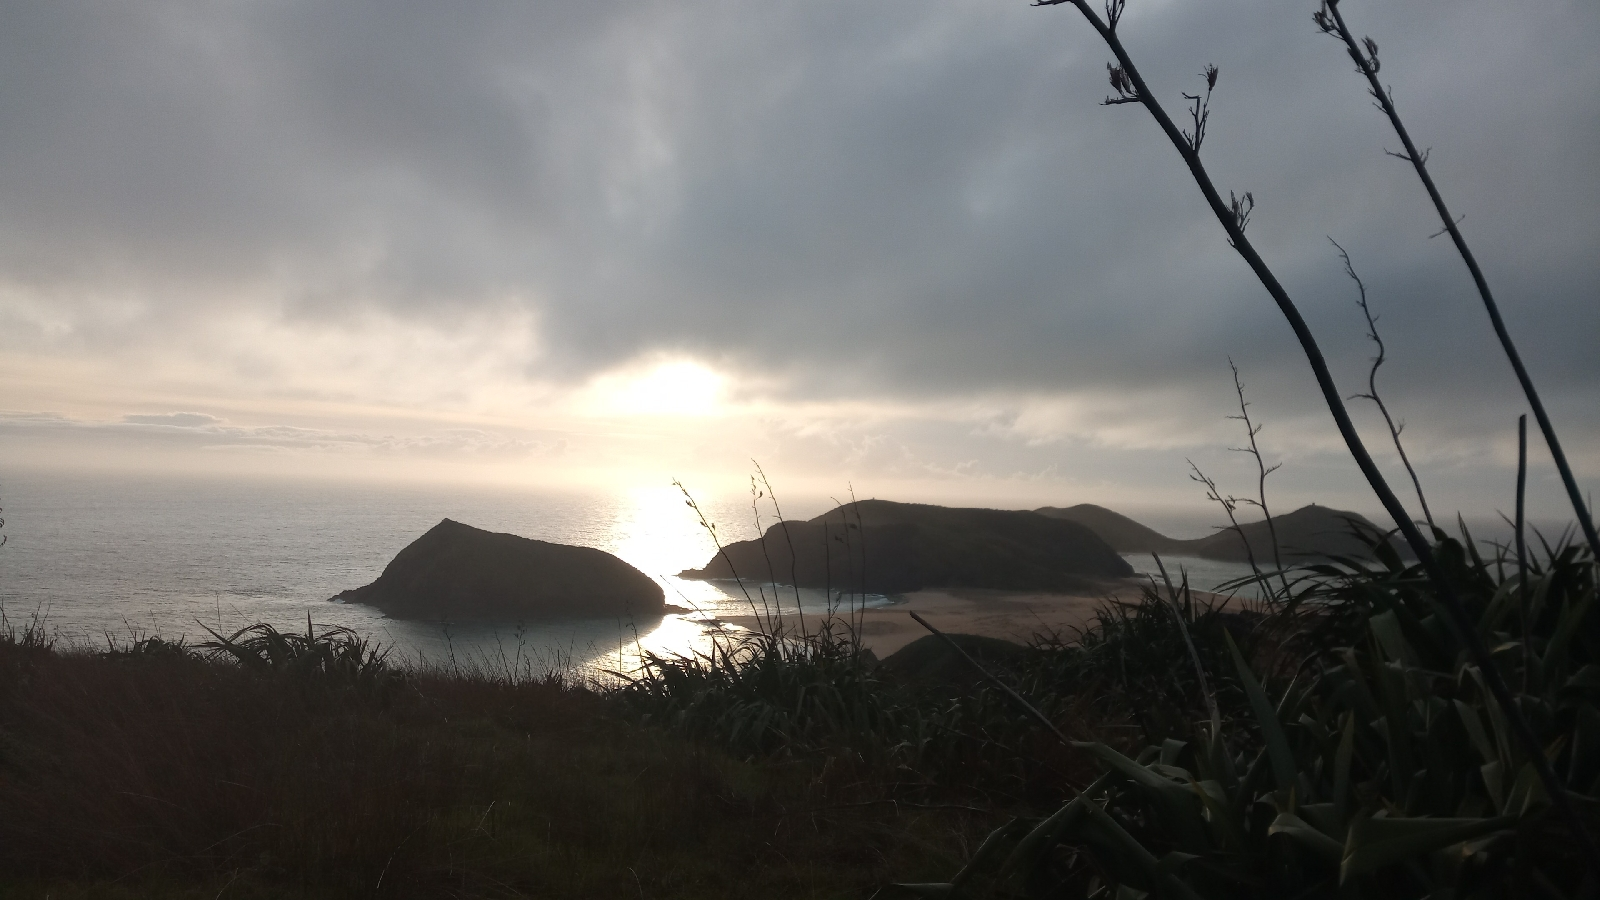
\includegraphics[width=0.5\textwidth]{der_anfang_doch_wie_kommt_man_dahin/24_1666211231105337-8.png}
	\caption{}
	\label{fig:24_1666211231105337-8}
\end{figure}

\begin{figure}[H]
	\centering
	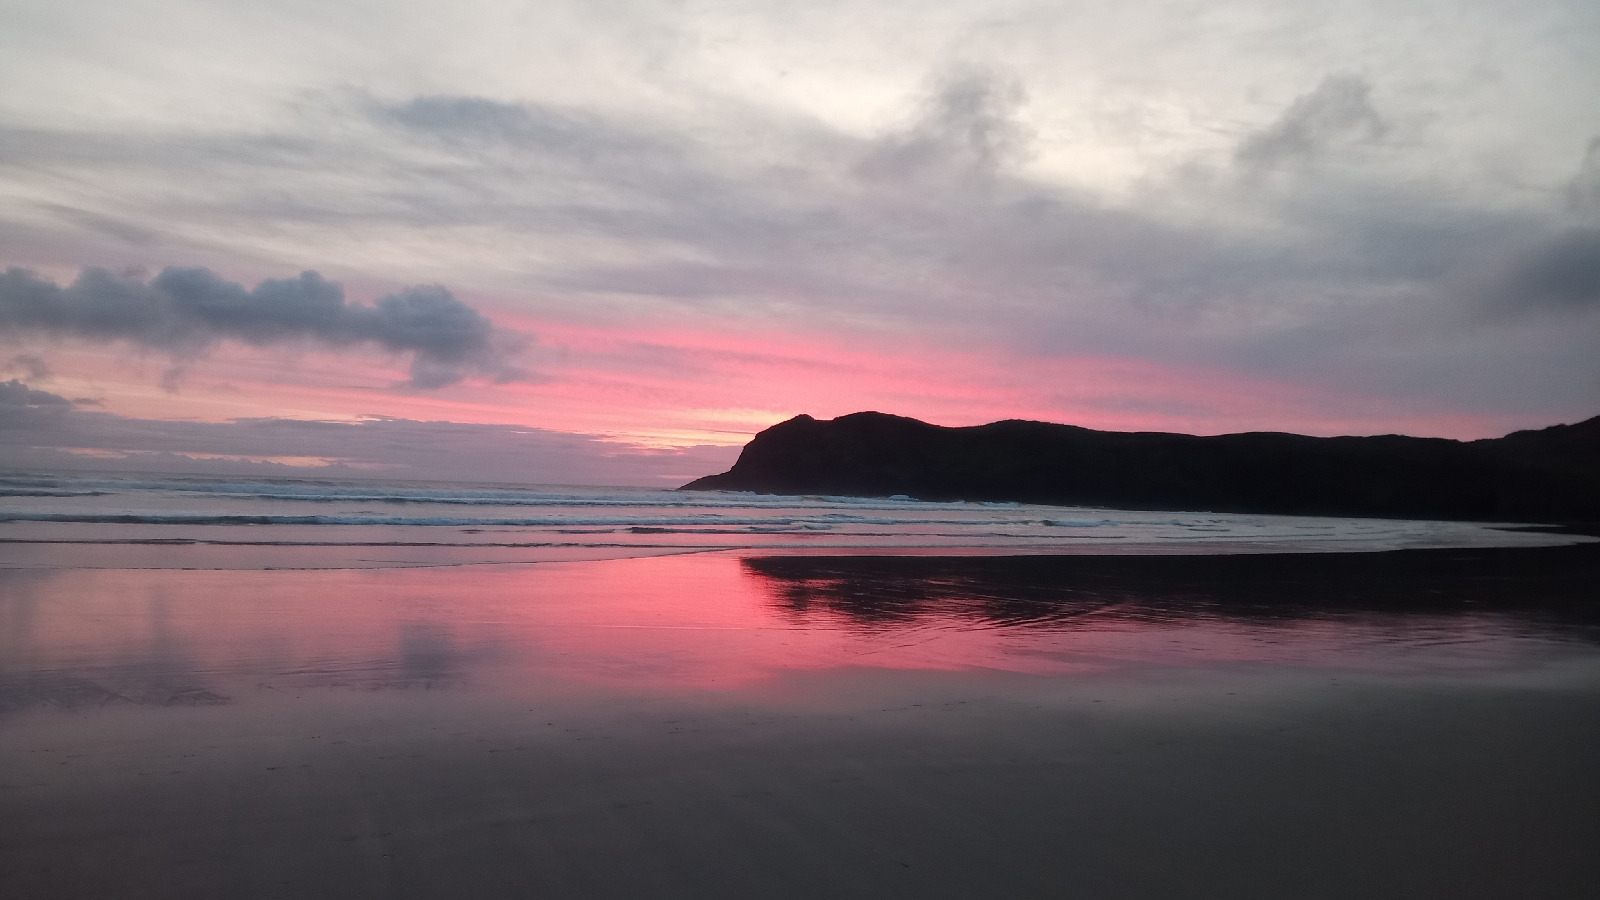
\includegraphics[width=0.5\textwidth]{der_anfang_doch_wie_kommt_man_dahin/25_1666211225753094-9.png}
	\caption{}
	\label{fig:25_1666211225753094-9}
\end{figure}

  Und auch dieses Mal holt uns die Dunkelheit ein, mit Stirnlampen auf dem Kopf erreichen wir gegen 20:30 das Camp. Im Dunkeln bauen wir schnell unser Zelt auf, um schon etwa eine halbe Stunde später die Augen zu schließen. Die Küche blieb wieder ein Mal kalt.
 


  gelaufenen KM 12,5
 


   Di 18.10.22    Tag 2
  


   Twilight Beach Camp - Bluff Campsite
  


  Km 12,5 - 40,3
 


  Bei Tageslicht erkennen wir erst die große Anzahl an Zelten auf dem Platz. 11 Zelte und etwa genau so viele Wander zählen wir.
 


\begin{figure}[H]
	\centering
	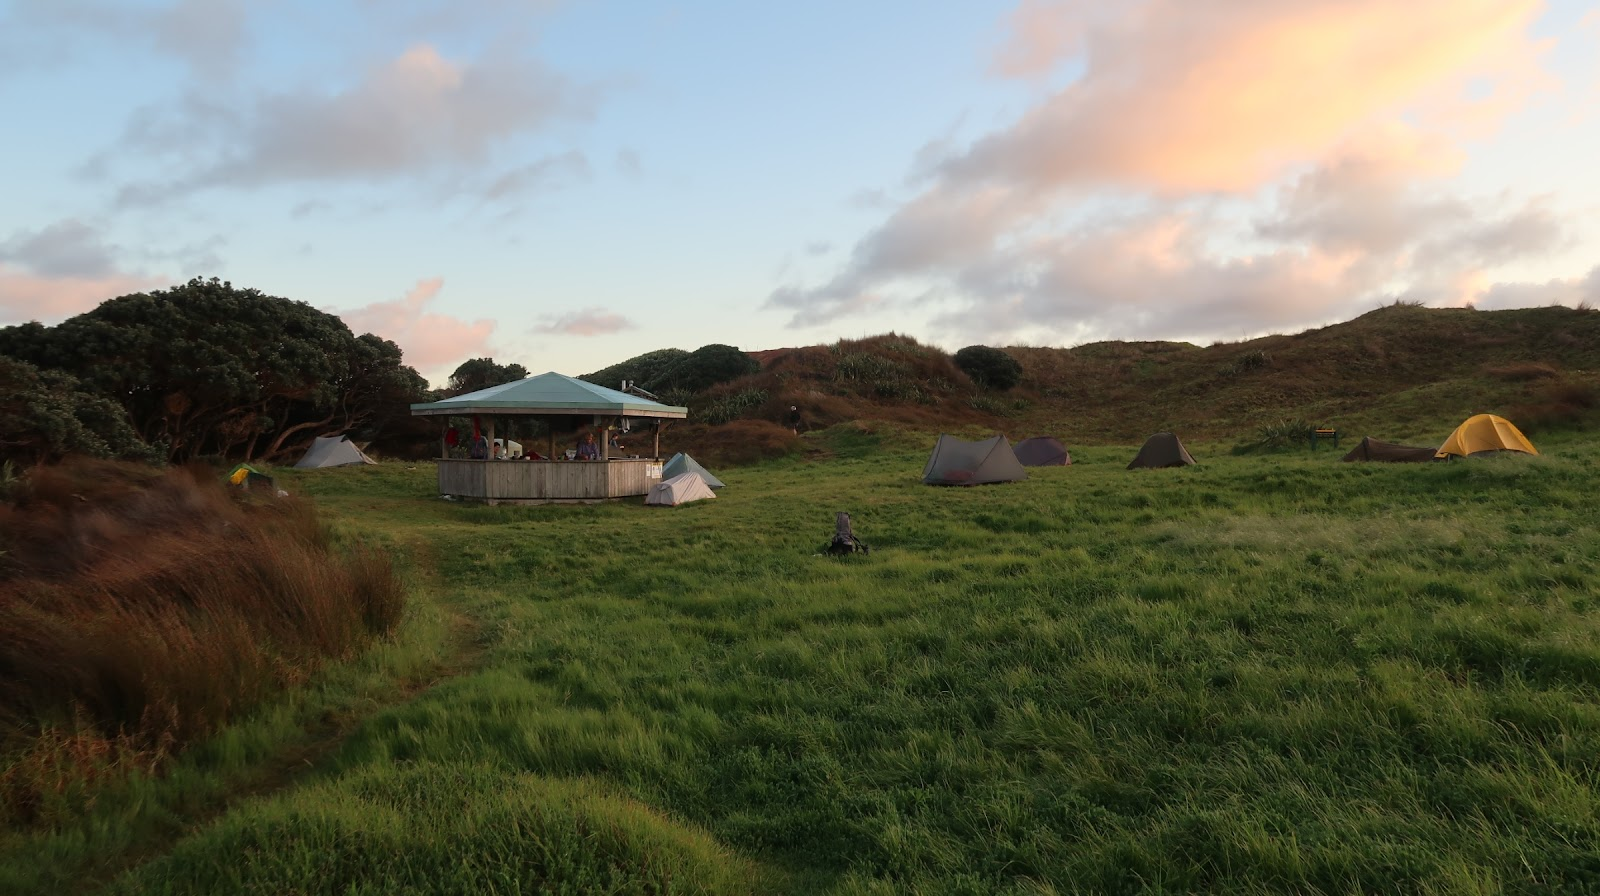
\includegraphics[width=0.5\textwidth]{der_anfang_doch_wie_kommt_man_dahin/26_1666211218139811-10.png}
	\caption{}
	\label{fig:26_1666211218139811-10}
\end{figure}

\begin{figure}[H]
	\centering
	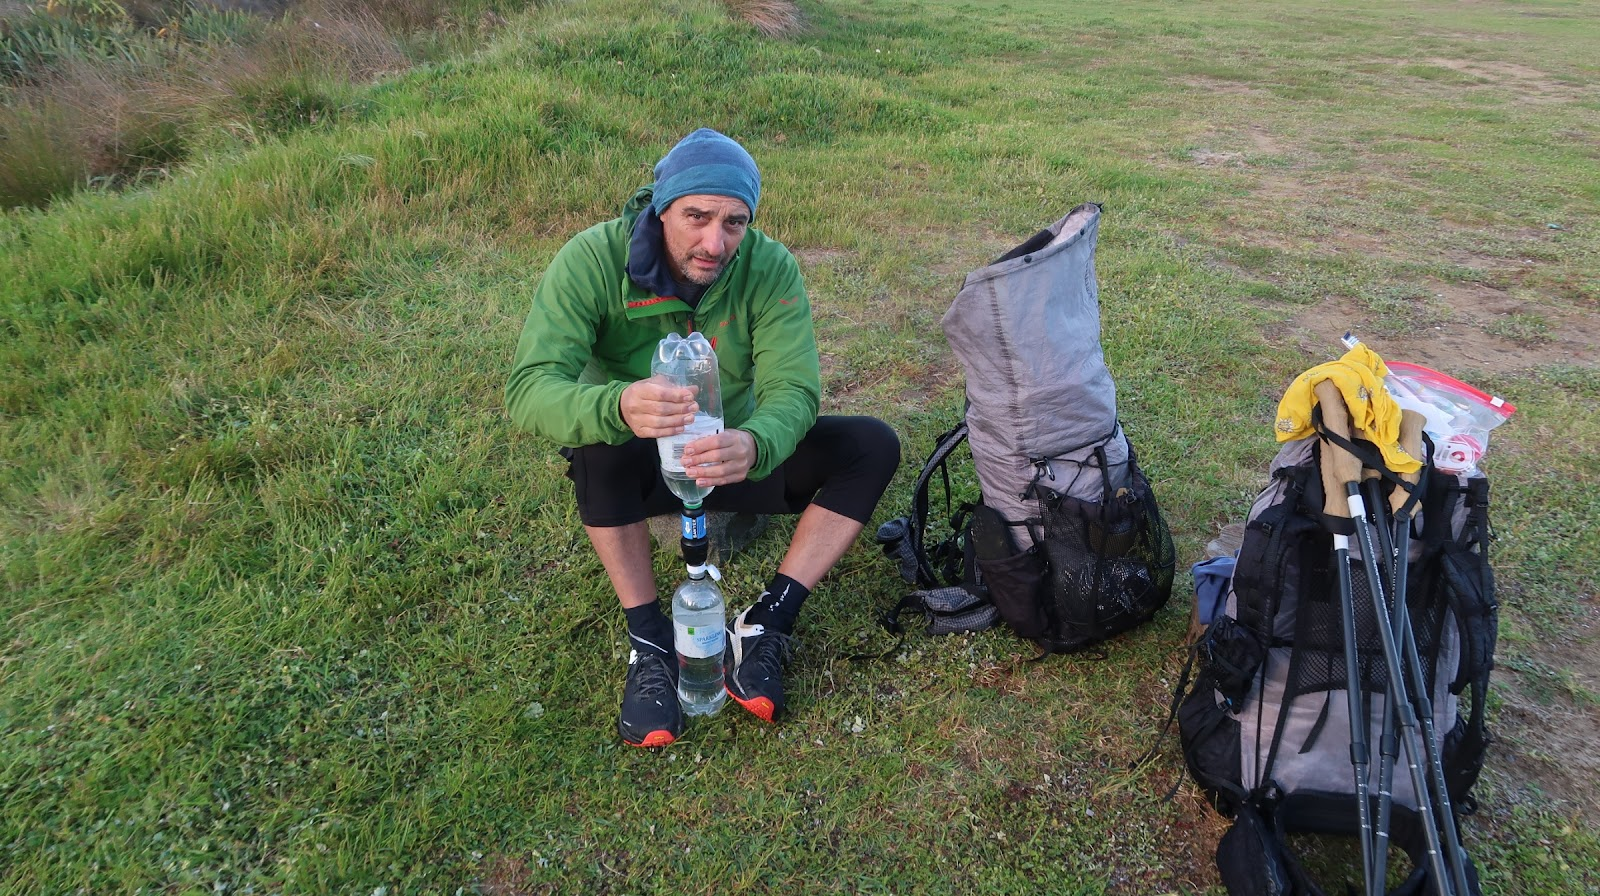
\includegraphics[width=0.5\textwidth]{der_anfang_doch_wie_kommt_man_dahin/27_1666211193312039-11.png}
	\caption{}
	\label{fig:27_1666211193312039-11}
\end{figure}

\begin{figure}[H]
	\centering
	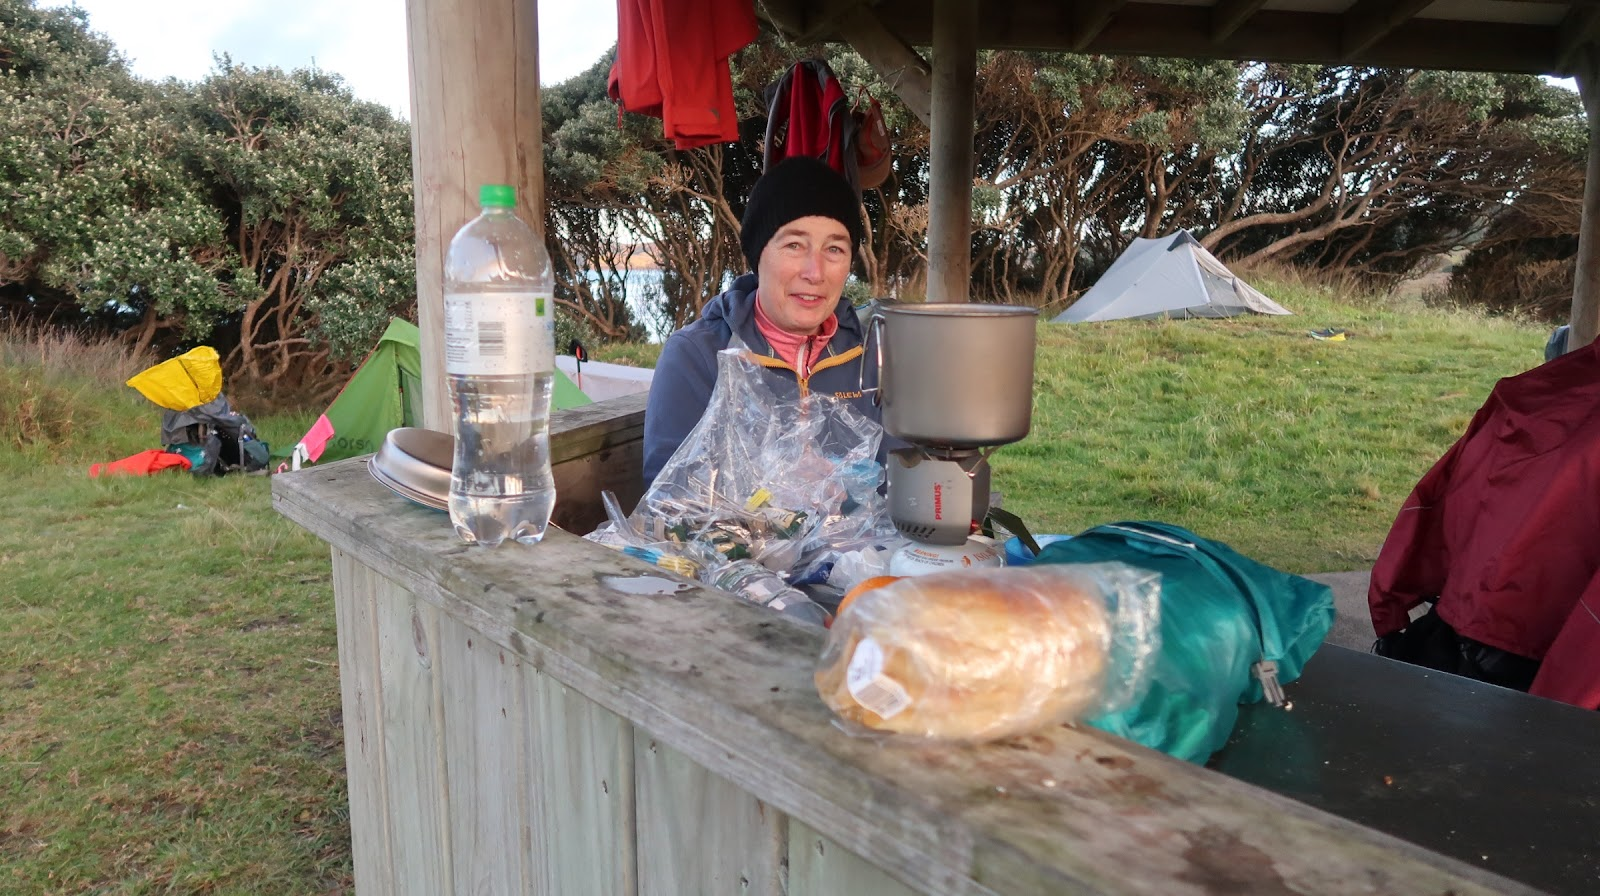
\includegraphics[width=0.5\textwidth]{der_anfang_doch_wie_kommt_man_dahin/28_1666211181538298-12.png}
	\caption{}
	\label{fig:28_1666211181538298-12}
\end{figure}

\begin{figure}[H]
	\centering
	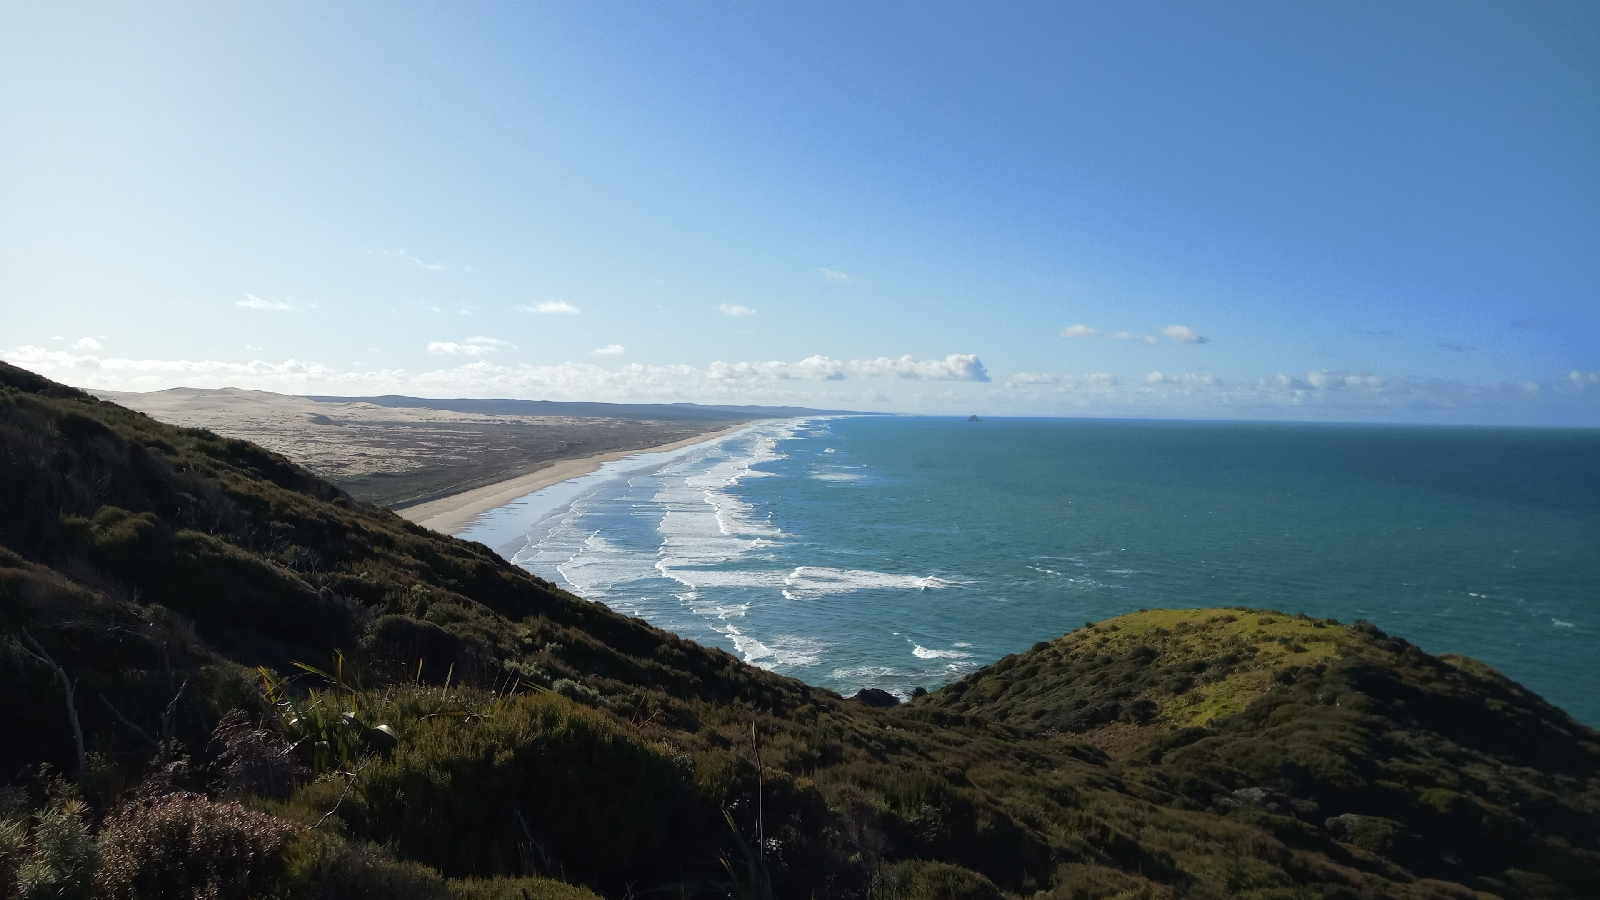
\includegraphics[width=0.5\textwidth]{der_anfang_doch_wie_kommt_man_dahin/29_1666211175152805-13.png}
	\caption{}
	\label{fig:29_1666211175152805-13}
\end{figure}

  gelaufene KM 27,8
 


    Mi 19.10.22    Tag 3
   


    Bluff Campsite - Hukatere Campsite
   


   Km 40,3 - 70,1
  


  Der heutige Tag ist schnell erzählt,  rechts Brandung, links Dünen, in der  Mitte wir.
 


\begin{figure}[H]
	\centering
	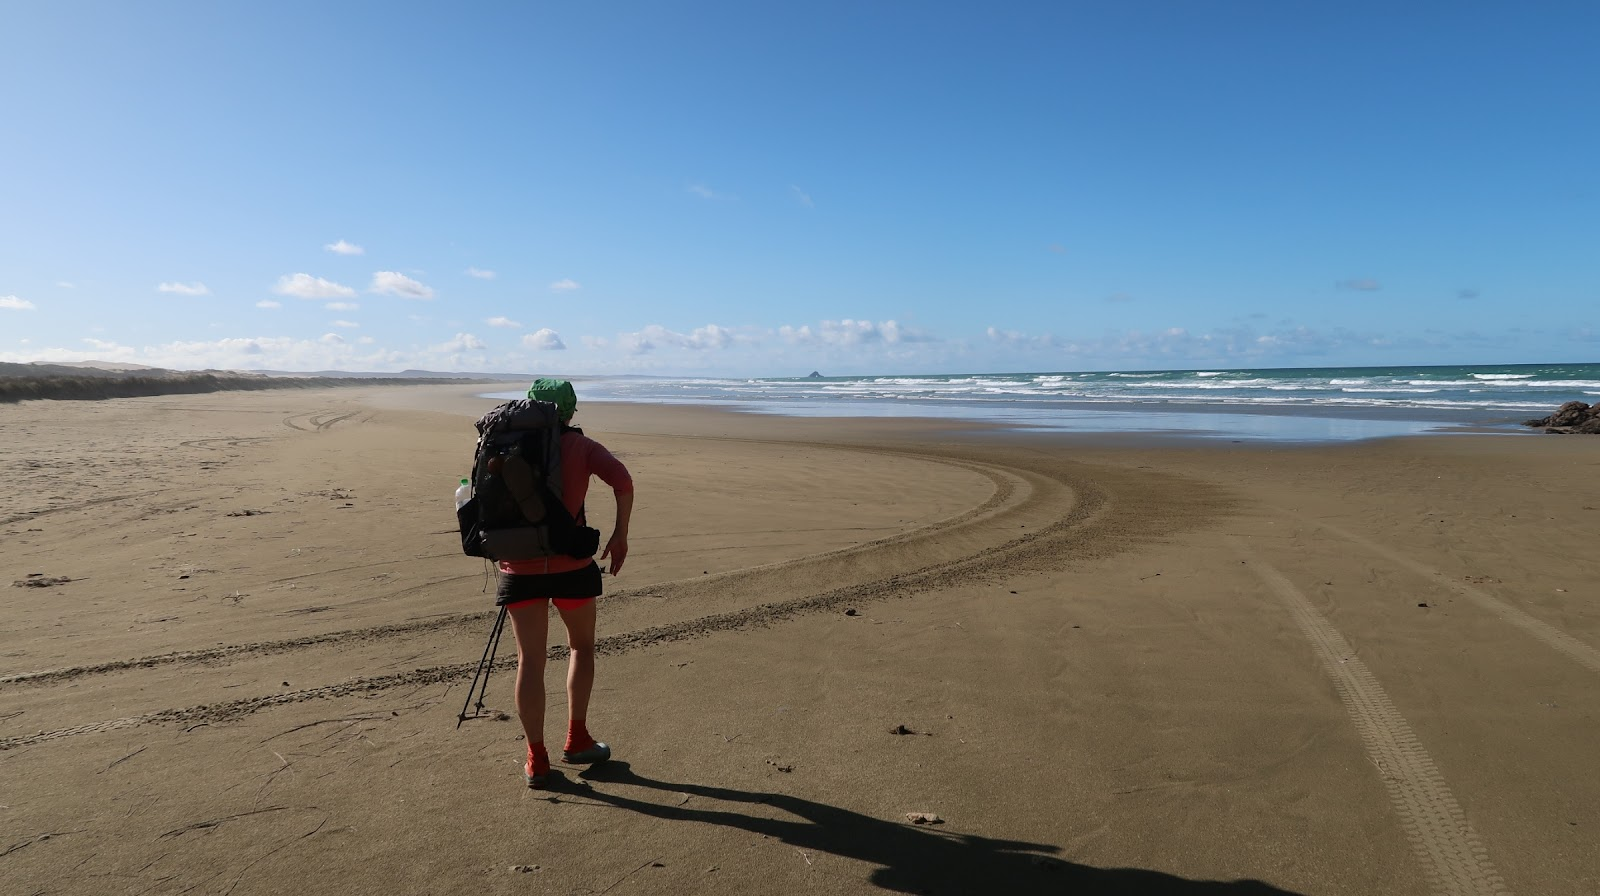
\includegraphics[width=0.5\textwidth]{der_anfang_doch_wie_kommt_man_dahin/30_1666211167568198-14.png}
	\caption{}
	\label{fig:30_1666211167568198-14}
\end{figure}

  Mit einem super Ausblick auf das Meer.
 


\begin{figure}[H]
	\centering
	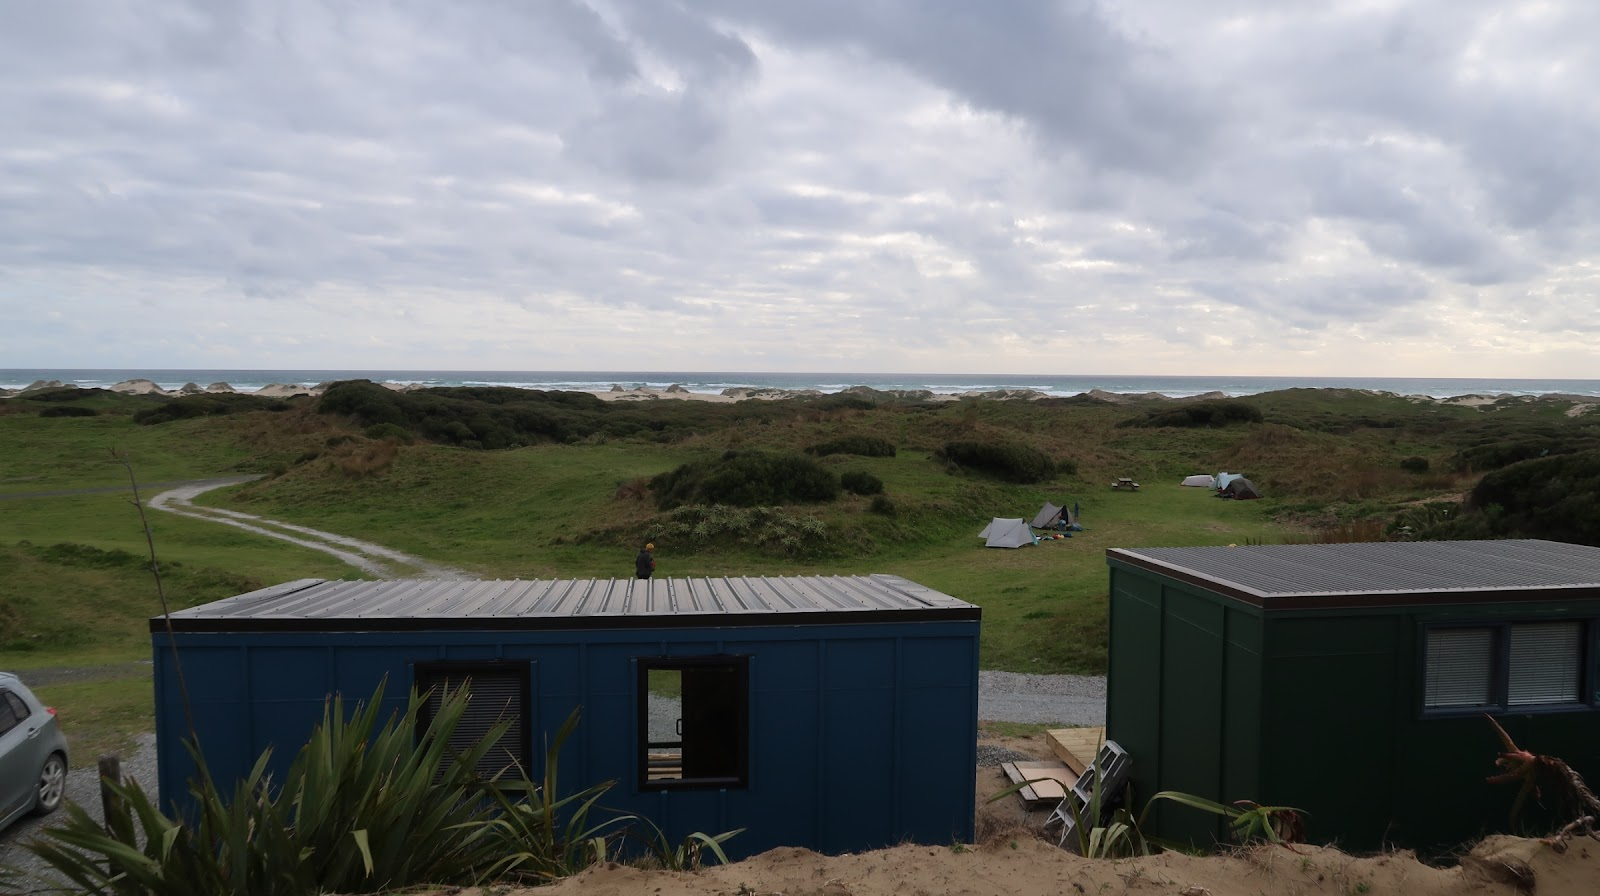
\includegraphics[width=0.5\textwidth]{der_anfang_doch_wie_kommt_man_dahin/31_1666211159419889-15.png}
	\caption{}
	\label{fig:31_1666211159419889-15}
\end{figure}

  gelaufene Km 29,8
 

